\chapter{多人合乘情境下求解乘载最多乘客}
\label{chap:ridesharing}

在上一个章节,我们考虑了两个出行合乘,并且每个出行都只有一个乘客的情形。但是,实际当中,我们可以允许很多人一起乘车,两个以上的出行进行合乘也是可行的。在现有的出租车中,车的座位数量都为4座,两个人合乘显然仍然有很多的座位被浪费,因此,在实际中,考虑多个出行进行合乘的情形也十分的必要。在上一章节中,我们为了简化问题的讨论,仅考虑了两人合乘的简单情形,在这一章节,我们将进一步讨论多个出行进行合乘的情况。也就是说,在这里,我们将不限定进行合乘的出行的数量为某一个特定的值,而是在满足车的容量限制下的大于2的任意值。例如,如果车的座位数量为4,则两个出行,三个出行,四个出行都可以进行合乘。
\par
具体来说,我们在这里要考虑的问题是:在已知车辆的位置的情况下,如何将现有的出行进行合乘,并且给合乘的出行进行车辆的分配。因为,需要已知车辆的座位数量,才可以将车辆和出行进行匹配,所以,我们需要预先知道车辆的物理信息。在进行匹配的过程中,我们需要考虑车辆和合乘后的出行的时空信息的匹配程度,所以我们也需要预先知道车辆的时空信息。在这样的情景设定下,我们考虑的目标,不再是求解最小的车辆规模,因为车辆的信息我们需要预先知道。在这里,我们考虑的目标是在给定车的数量的情况下最大化服务的乘客的数量。
% 但是实际当中,出行的乘客很多情形下都不止一个,比如一家人去火车站或者机场准备出远门,朋友们一起坐车出去看电影或者游玩,公司聚会坐车去饭店等。

\section{数学规划模型}
在这一部分,我们将利用数学规划将问题进行数学建模。在进行建模之前,我们先给出一些基本的假设。
% \subsection{基本假设}
\begin{enumerate}
\item 我们仅考虑充分短的时间段内的车辆,即,在我们考虑的时间段内,没有i虚拟的车辆到达,只有在时间开始时的车辆可供分配调度。
\item 对于每一个我们考虑的乘客,如果乘客在与他人合乘的过程中的收益大于损失,并且损失在可接受的范围内,则这位乘客将会选择合乘。
\item 对于一名车的司机而言,如果合乘时绕路的长度在他可接受的范围内,并且他的收益至少为他在不进行合乘时驾驶相同的距离和时间所得到的收益的均值,则他愿意提供合乘服务。
\end{enumerate}

\par
接下来是一些主要的记号。
\begin{longtable}{|r|l|}
        \caption{主要的记号}
            \label{tab:not}\\	
    \hline
       记号  & 含义 \\
       \endfirsthead
       记号 & 含义 \\
		\hline
		\hline
		\endhead
		\bottomrule \multicolumn{2}{r}{\textit{接下一页}} \\
		\endfoot
		\endlastfoot
       \hline
       \hline
        $\mathcal{P}$ & 乘客的全体组成的集合\\
        \hline
        $N_i$ & “邻近”(见定义~\ref{def:close})乘客$i$的左右乘客组成的集合\\
        \hline
        $\mathcal{O}$ & 出发点集合\\
        \hline
        $\mathcal{D}$ & 目的地集合\\
        \hline
        $\mathcal{DT}$ & 出发时间集合\\
        \hline
        $\mathcal{AT}$ & 最晚到达时间集合\\
        \hline
        $G_i$ & 由包含乘客$i$的两两临近的乘客组成的集合\\
        \hline
        $M_i$ & 乘客$i$可能可以合乘的出行集合\\
        \hline
        $Loss_i^m$ & 乘客$i$加入合乘$m$的损失\\
        \hline
        $\mathcal{O}_f^m$ & 合乘$m$的最终出发地点\\
        \hline
        $\mathcal{D}_f^m$ & 合乘$m$的最终到达地点\\
        \hline
        $\mathcal{DT}_f^m$ & 合乘$m$的最终出发时间\\
        \hline
        $\mathcal{AT}_f^m$ & 合乘$m$的最终到达时间\\
        \hline
        $\mathcal{M}$ & 所有的合乘组成的集合\\
        \hline
        $Dis_i^m$ & 乘客$i$加入合乘$m$所能得到的折扣\\
        \hline
        $Pay_i^m$ & 乘客$i$加入合乘$m$后应当付给司机的钱\\
        \hline
        $f_i$ & 乘客$i$在不合乘的情况下应当付的路费\\
        \hline
        $\delta$ & 在定义“邻近”中的常数距离阈值\\
        \hline
        $t$ & 在定义“邻近”中的常数时间阈值\\
        \hline
        $\Delta _m$ & 与合乘$m$匹配的司机在不提供合乘服务时,在这种情境下能够得到的收入的均值\\
        \hline
        $r_m$ & 合乘$m$中的所有乘客\\
        \hline
        $c_i^m$ & 指示变量, 当乘客$i$加入合乘$m$时为1,否则为0\\
        \hline
        $\zeta$ & 当选择合乘时,乘客所能接受的最大的损失\\
        \hline
        $\mathcal{B}$ & 可供调度的所有车辆组成的集合\\
        \hline
        $\overline{v}$ & 平均驾驶速度\\
        \hline
        $z_b^m$ & 指示变量, 当车$b$和合乘$m$匹配时为1,否则为0\\
        \hline
        $d_b^m$ & 车$b$为了接$m$所需要走过的距离\\
        \hline
        $\xi$ & 司机为了接一个合乘出行所能接受的最大的驾驶距离\\
\hline
\end{longtable}
其中,“邻近”的定义如下。
\begin{definition}[邻近]
对于乘客$i,j \in \mathcal{P}$,我们说他们是 彼此\textbf{邻近}的当且仅当$||\mathcal{O}_i - \mathcal{O}_j||_M \leq \delta $,$||\mathcal{D}_i - \mathcal{D}_j||_M \leq \delta$并且$|\mathcal{DT}_i- \mathcal{DT}_j| \leq t$,其中$||\cdot||_M$代表曼哈顿距离。
\label{def:close}
\end{definition}

\par
我们引进“邻近”的概念,是为了保证在一个合乘中的两个以及以上的乘客,在进行合乘时,不需要走很长的距离才能坐上车,或者需要等很长的时间才能等到车。当一个合乘中所有乘客都是两两邻近时,我们可以叫他们走到他们出发点的几何中心或者邻近的地方会和,一起上车。如果这样的条件不满足,则乘客可能并不会想和其他乘客一起合乘一辆车。
\[
\begin{aligned}
  \max & \sum_{b\in\mathcal{B}}\sum_{m\in\mathcal{M}} |r_m|z_b^m 
\end{aligned}
\]

\begin{align}
    s.t. \sum_{m\in M_i} c_i^m \leq&  1 \quad \forall i\in \mathcal{P}  \label{eq:c1}\\
    c_i^m =  & c_j^m \quad \forall i,j \in r_m \quad \forall m\in\mathcal{M} \label{eq:c2}\\
    \sum_{b\in\mathcal{B}}z_b^m \leq& 1 \quad \forall m\in\mathcal{M} \label{eq:c3}\\
    \sum_{m\in\mathcal{M}}z_b^m \leq& 1 \quad \forall b\in \mathcal{B} \label{eq:c4}\\
    d_b^m \leq& \xi \label{eq:c5}\\
    Loss_i^m \leq & Gain_i^m\quad \forall i\in\mathcal{P}, m \in \mathcal{M} \label{eq:c6}\\
    \Delta_m  \leq & \sum_{i\in r_m} Pay_i^m \quad \forall m \in \mathcal{M} \label{eq:c7}\\
    Loss_i^m \leq& \zeta \quad \forall i\in\mathcal{P},m\in\mathcal{M} \label{eq:c8}\\
    c_i^m, z_b^m&\in\{0,1\}\quad \forall i\in \mathcal{P}, b\in \mathcal{B}, m\in\mathcal{M} \label{eq:c9}
\end{align}

其中$Loss_i^m, Gain_i^m, Dis_i^m, f_i, \Delta_m$的定义如下:
\[
\begin{aligned}
Loss_i^m =& Function(||\mathcal{O}_i-\mathcal{O}_f^m||_M+||\mathcal{D}_i-\mathcal{D}_f^m||_M, |\mathcal{DT}_i-\mathcal{DT}_f^m|)\\
Gain_i^m = & Dis_i^m \cdot f_i\\
Dis_i^m = & Function(||\mathcal{O}_i-\mathcal{O}_f^m||_M+||\mathcal{D}_i-\mathcal{D}_f^m||_M, |\mathcal{DT}_i-\mathcal{DT}_f^m|, ||\mathcal{O}_i-\mathcal{D}_i^m||_M)\\
f_i = & Function(||\mathcal{O}_i-\mathcal{D}_i^m||_M)\\
\Delta_m = & Function(||\mathcal{O}_i-\mathcal{D}_i^m||_M,|\mathcal{DT}_f^m-\mathcal{AT}_f^m|)
\end{aligned}
\]
\par
这里,$Function$代表是函数。
\par
我们的目标函数是最大化车辆服务的乘客数量。约束\label{eq:c1}代表了,每个乘客最多只能乘一辆车,并且可能有一部分乘客没有车辆服务。约束\label{eq:c2}表示了合乘$m$的合理性。约束\label{eq:c3}和\label{eq:c4}表示了一辆车只能服务一个合乘,每个合乘只能和一辆车匹配。约束\label{eq:c5}和\label{eq:c7}保证了得到的解对司机是合理的,约束\label{eq:c6}和\label{eq:c8}保证了合乘对于合乘中每一个乘客都是合理的。约束\label{eq:c9}说明了优化问题是一个0-1整数规划问题。

\section{证明问题为NP-hard}
以下我们证明,以上我们用混合整数规划建模的问题是NP-hard的问题。我们将原问题规约为一个NP-Complete问题——Complete Coloring。
\par
从图论的语言,我们可以将Complete Coloring表述如下。
\par
\textit{给定一个图$G = (V,E)$和一个整数$k$,回答问题:是否存在一个对$V$的划分,将$V$划分为$k$或者更多的两两不交的子集合$V_1,V_2,\cdots,V_k$,使得$\forall i=1,2,\cdots,k, V_i$都是$G$上的独立集,并且$\forall i\neq j, V_i\cup V_j$不是$G$的独立集。
}
\par
在证明之前,我们先引入两个定义。
\begin{definition}[稳定对]
两个乘客$i,j\in\mathcal{P}$ are a \textbf{稳定对}当且仅当他们是互相邻近的,并且$Gain^m_i\geq Loss^m_i, Gain^m_j\geq Loss^m_j  \quad\forall m\in M_i\bigcap M_j$ 。
\end{definition}
\begin{definition}[稳定组]
一组乘客是一个\textrm{\textbf{稳定组}}当且仅当他们两两构成\textrm{稳定对}。
\end{definition}
\begin{theorem}
原问题可以规约为Complete Coloring问题,从而原问题是NP-hard的问题。
\end{theorem}
\begin{proof}
任意给定一个Complete Coloring的问题的实例,我们可以通过如下的方法构造我们的问题的一个实例。
\par
\textit{
记$P$为所有乘客的集合,乘客$p_i$为一个节点,对于每对不能形成稳定对的乘客,我们在他们的节点之间加一条边。假设对于任意的$b\in \mathcal{B}$,它可以乘载他们中的任何一个,并且车的容量足够大。
}
\par
\textit{
我们可以构建如下的映射:我们将$G$中的每一个节点$v_i$对应为$p_i\in P$的节点,并且让独立集$V_i$视为$b_i\in\mathcal{B}$中的车。我们可以观察到,可以构成稳定组的乘客可以被视为yyi一个独立集。所以有相同颜色的节点形成一个稳定组,并且与一个车匹配。车中的乘客的集合是图中的一个独立集。显然,如果我们的问题有一个解,即,存在车辆和合乘后的出行的一个匹配,则Complete Coloring问题也可解。如果存在$G$的一个满足如前所述的性质的划分,则存在一个车辆和出行匹配。
}
\end{proof}

\section{一个基于图论的精确算法}
在给出了稳定对和稳定组的定义之后,我们可以根据乘客之间的相互关系生成图。图中的每一个节点代表一个乘客,如果两个乘客之间可以合乘,我们就将他们之间加一条边。算法如算法~\ref{alg:ocnstruct}。
\begin{algorithm}[htbp]
 \SetAlgoLined
\SetKwInOut{Input}{Input}\SetKwInOut{Output}{Output}
\caption{VehicleTripGraph($G$)}
\label{alg:construct}
\BlankLine
$\mathcal{T}\leftarrow \emptyset$;$\quad$ $\mathcal{E}\leftarrow \emptyset$;\quad $\mathcal{T}_i \leftarrow \emptyset ,i=1,2,\cdots,\nu$\;

    % \For{$i$从1到$\nu$}{
    %     $\mathcal{T}_i\leftarrow \emptyset$\;
    % }
    \For{$e = (b,v)\in G$}{
        $\mathcal{T}_1\leftarrow \mathcal{T}_1\bigcup \{v\}$;\quad$\mathcal{E}\leftarrow \mathcal{E}\bigcup \{(b,v)\}$\;
    }
    \For{$\forall v_1,v_2\in \mathcal{T}_1$ and $e = (v_1,v_2)\in G$}{
        $T \leftarrow\{v_1,v_2\}$\;
        $\mathcal{T}_2\leftarrow \mathcal{T}_2\bigcup T$;\quad$\mathcal{E}\leftarrow\mathcal{E}\bigcup \{(v_1, T),(v_2,T)\}$\;
        \If{$(b,v_1),(b,v_2)\in G$}{
            $\mathcal{E}\leftarrow\mathcal{E}\bigcup \{(b,T)\}$\;
        }
    }
    \For{$j$从$3$到$\nu$}{
        \For{$\forall T_1,T_2\in \mathcal{T}_{j-1}$和$|T_1\bigcup T_2| = j$}{
            记$T_1\bigcup T_2 = \{v_1,v_2,\cdots,v_j\}$\;
            \If{$\forall k \in \{1,2,\cdots,j\}, \{v_1,v_2,\cdots,v_j\}\backslash v_k\in \mathcal{T}_{j-1}$}{
                $T\leftarrow T_1\bigcup T_2$\;
                \For{$i$从1到$j$}{
                	$\mathcal{E}\leftarrow \mathcal{E}\bigcup \{(v_i,T)\}$\;
                }
                \If{$b$可以加入$T$}{
                    $\mathcal{T}_j\leftarrow \mathcal{T}_j\bigcup T$;\quad$\mathcal{E}\leftarrow \mathcal{E}\bigcup \{(b,T)\}$\;
                }
            }
        }
    }
    $\mathcal{T}\leftarrow (\bigcup_{i\in\{1,\cdots,\nu\}}\mathcal{T}_i)\bigcup\mathcal{T}$\;
\For{每一个$b\in\mathcal{B}$}{
    \For{$t\in \mathcal{T}$}{
        \If{$b$可以与合乘$t$匹配}{
            $\mathcal{E}\leftarrow\mathcal{E}\bigcup \{(b,t)\}$
        }
    }
}
\end{algorithm}
\par
基于此算法生成的网络,我们使用动态规划的方法进行求解,我们根据动态规划提出算法~\ref{alg:optimal}。

\begin{algorithm}[htbp]
 \SetAlgoLined
\SetKwInOut{Input}{Input}\SetKwInOut{Output}{Output}
\caption{Optimal($G$)}
\label{alg:optimal}
\BlankLine
求得所有的连通分支集合$\mathcal{C}$\;
\eIf{$|\mathcal{C}| > 1$}{
    $\mathcal{W}\leftarrow \emptyset$\;
    $\mathcal{S}\leftarrow \emptyset$\;
    \For{$c\in \mathcal{C}$}{
        $w_c,s_c\leftarrow \texttt{Optimal}(G_c)$\;
        $\mathcal{W}\leftarrow\mathcal{W}+w_c $\;
        $\mathcal{S}\leftarrow\mathcal{S}\bigcup s_c $\;
    }
}{
    对$\mathcal{E}$中的所有边从$1$ 到 $n = |\mathcal{E}|$进行编号\;
    $e_1 = (u_1,v_1)\leftarrow$记为$\mathcal{E}$中的第一条边\;
    $G_1\leftarrow G$ 去除 $e_1$\;
    $G_2\leftarrow G$ 去除 $e_1,u_1,v_1$,所有$u_1$的出弧和所有$v$的入弧和它的邻居节点\;
    \For{$v\in\mathcal{V}_2$}{
        \If{$u\cap u_1 != \emptyset$}{
            删除$u$和它在中$G_2$的入弧\;
        }
    }
    $\mathcal{W}_1,\mathcal{S}_1\leftarrow \texttt{Optimal}(G_1)$;$\quad$ $\mathcal{W}_2,\mathcal{S}_2\leftarrow \texttt{Optimal}(G_2)$\;
    \eIf{$\mathcal{W}_1 > \mathcal{W}_2$}{
        return $\mathcal{W}_1, \{s_1 = 0\}\bigcup\mathcal{S}_1$\;
    }{
        return $\mathcal{W}_2, \{s_1 = 1\}\bigcup\mathcal{S}_2$\;
    }
}
\end{algorithm}

\par
为了证明我们算法的正确性,即算法的返回值和我们在上一部分提出的数学规划的解是一致的,我们将其写为一个定理。
\begin{theorem}
算法~\ref{alg:optimal}~可以返回整数规划的最优解。
\end{theorem}

\begin{proof}
首先,我们证明算法~\ref{alg:optimal}~的解满足整数规划的约束。
\begin{enumerate}
\item 当一辆车在算法执行过程中被选择了,即存在它的一条出弧$e_i\in \mathcal{E},s_i = 1$,那么它将会在之后的过程中被选择,因为它的所有出弧都在它被选择匹配之后就被删除,所以一辆车只能和一个合乘出行匹配。
\item 只要对一条边$e_i,s_i=1$,那么被匹配的出行的入弧和它的邻接节点都将从图$G$中被删除,所以一个合乘出行只能和一辆车进行匹配。
\item 当删除一个合乘出行的所有的入弧时,算法会探查到和这个出行不相容的出行,这些出行将会被算法从$G$中删除。这里的不相容是指,它们中包含相同的原始的出行。因此,每个原始的出行都在得到的解中只会出现在一个合乘出行里。
\end{enumerate}
\par
其次,我们证明算法的结果是最优的。我们利用反证法。
\par
假设有一个整数规划的最优解不能被算法~\ref{alg:optimal}~返回。假设被选择的边的编号为$e_{n_1},e_{n_2},\cdots,e_{n_k}$,即$s_{n_i}=1,\forall i\in \{1,2\cdots,k\}$将会被算法返回。那么,我们来考虑在求解过程中算法的执行过程。
\par
第一步,$s_1 = 0$或者1被选择。如果$s_1 = 0$,那么只有一条弧被删除,算法将会继续选择$s_2$的值。如果$s_2 = 0$,那么算法将会选择$s_3$的值。以此类推。当算法到达需要决定$s_{n_1}$的值的时候,0和1都是可能的选择。当$s_{n_1}=1$将会被探索时,算法将会考虑$s_{n_1+1},\cdots,s_{n_2-1}$的值。算法将$s_k=0\forall k\in \{n_1+1,\cdots,n_2-1\}$,列入算法的搜索空间中。只要算法将$s_{n_1+1},\cdots,s_{n_2-1}$赋值为0,这样的赋值就会被返回,然后算法就会选择$s_{n_2}$的值。以此类推,直到算法选择$s_{n_k}=1$,此时算法结束,因为所有的弧都被删除,这一条分支完成。
\par
从以上可以看出,赋值$s_{n_1},\cdots,s_{n_k}=1$被包含在算法的搜索空间中,因此,如果这个解是最优解并且是唯一的,算法一定会返回这个解,如果是最优的但是不是唯一的最优解,算法返回的解一定不会比这个解差,所以也是最优解。
\par
综上所述,算法返回的一定是最优解。
\end{proof}

\section{算法执行过程的一个示例}
考虑图~\ref{fig:demovtg}~中的匹配。左边红色的节点代表车辆,右边的节点代表可能的合乘。我们利用算法~\ref{alg:optimal}~求解的过程如图~\ref{fig:demo}。算法的具体执行过程如下。
\begin{itemize}
\item[第一步] 从上到下给节点编号为$1,2,\cdots,12$。
\item[第二步] 当$s_1=1$时,车$b_1$和出行1号匹配,1号出行中包含了乘客1号。
\item[第三步] 这时我们需要考虑第二辆车,如果$s_{10}=1$,则算法结束。
\item[第四步] 如果$s_{10}=0$,则算法将会考虑$s_{11}$的取值。如果$s_{11}=1$,则算法执行结束。
\item[第五步] 如果$s_{11}=0$,则算法将会考虑$s_{12}$的取值,如果$s_{12}=1$,则这条路径结束。
\item[第六步] 如果$s_{12}=1$,则此时的解不是最优解,事实上,这个解是不可行的解,因为车辆$b_2$可以乘载乘客,但是在这个解里,它并没有。
\end{itemize}
\par
算法像如上过程执行,直到所有的可能性都被发掘。最终返回的结果是使得被服务到的乘客数量最大的解。

\begin{figure}
\centering
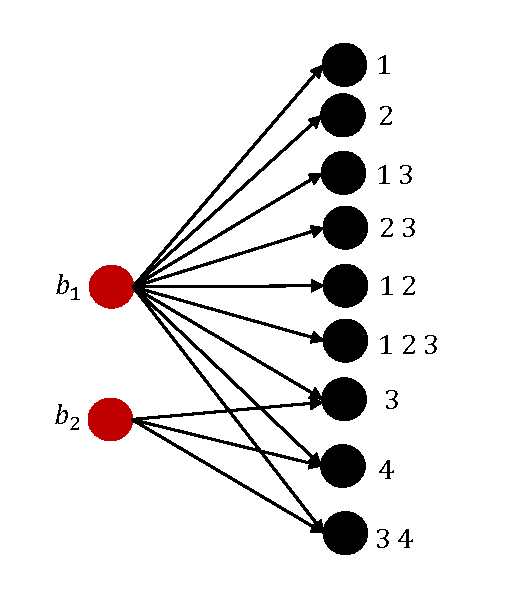
\includegraphics[width=10cm]{./figures/img/VTG.pdf}
\caption{一个示例}
\label{fig:demovtg}
\end{figure}


\begin{figure}
\centering
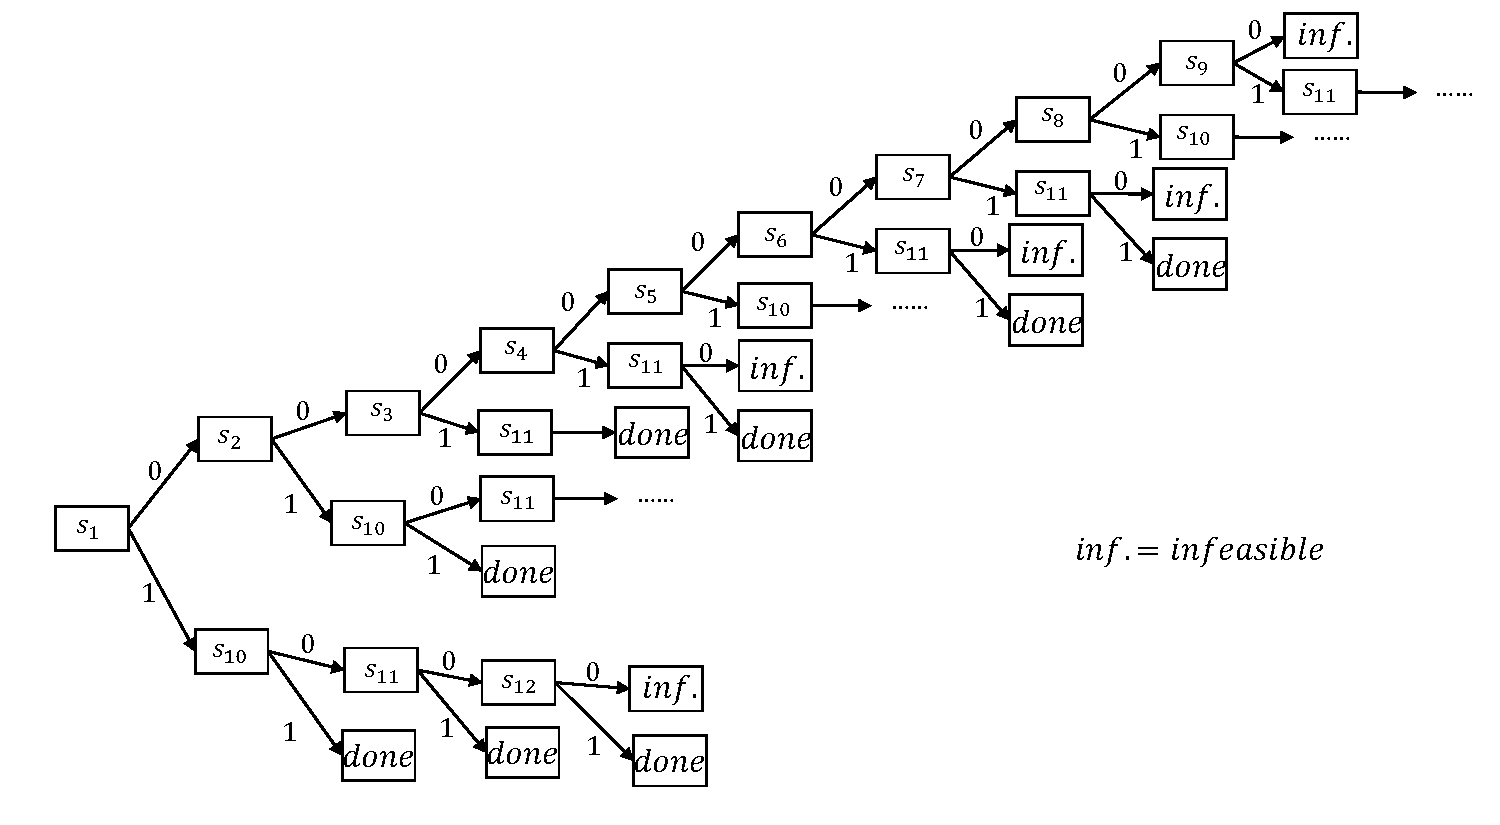
\includegraphics[width=15cm]{./figures/img/Demo_1.pdf}
\caption{算法执行过程示例}
\label{fig:demo}
\end{figure}


\section{算法时间复杂度分析}
从算法的执行过程中,我们可以得到算法~\ref{alg:optimal}~的时间复杂度的递推公式可以携程如下的形式:
\begin{equation}\label{eq:complex}
    T(|\mathcal{E^\prime}|) = T(|\mathcal{E^\prime}| - 1) + T(|\mathcal{E^\prime}| - d_b-\sum_{i = 0}^{d}d_{v_i} +d+1) + O(|\mathcal{B^\prime}|-1+|\mathcal{V^\prime}|-d-1)
\end{equation}
\par
其中$d_b,d_{v_i},d$分别代表被选择的节点的出度,入度,以及邻接节点的数量。$\mathcal{E}^\prime,\mathcal{V}^\prime,\mathcal{B}^\prime$分别代表当前边,当前出行节点,当前车辆节点。
\par
下面,求解此方程的方法展示如下。
\begin{itemize}
	\item[情形1] 当$d=0$时,即所有的合乘出行都只有一个原始出行。则问题可以被改变为最大二分匹配问题,这可以用匈牙利算法或者Hopcroft-Karp算法在多项式时间内求解。
	\item[情形2] 如果一个车辆只和形成一个稳定组的出行有边相连,则我们可以直接将车分配给该节点,这个节点包含了最多的原始出行,最多的乘客。这也可以在多项式时间内完成。
	\item[情形3] 当以上情形都不成立时,我们可以对$- d_b-\sum_{i = 0}^{d}d_{v_i} +d+1$给出一个估计。因为$d_b\geq 6, \sum_{i = 0}^{d}d_{v_i}\geq 2 (d+1),d\geq1$,那么$d_b+\sum_{i = 0}^{d}d_{v_i} -d-1\geq 8$。最差情况下,$d_b+\sum_{i = 0}^{d}d_{v_i} -d-1= 8$。在这样的情形下,为了求解原始的递推公式,我们只需要求解以下的方程:
	\begin{equation}
        x^8 = x^7 +1
    \end{equation}
    \par
    这个方程的一个实根为$x = 1.2321$。因为方程~\ref{eq:complex}~的最后一项只在现在探索的边选择为1时出现,并且在最终的解中,被选择为1的边的数量不超过车辆的数量。另外,这个附加项在一条边的$s$被指定为1时会减小,因此,附加项的时间复杂度为$O(|\mathcal{B}|^2)$。
    \par
    综上所述,算法~\ref{alg:optimal}~的时间复杂度为$O(1.2321^{|\mathcal{E}|}+|\mathcal{B}|^2)$。

\end{itemize}


\section{数据实验}
\subsection{数据来源}
本实验的数据来源于New York City Taxi \& Limousine Commission 上提供的公开数据集。数据中包含一次出行的出发地点,到达地点,出发时间,到达时间。在实验中,我们将选择不同大小的数据集以评价算法的效率。
\subsection{实验结果}
所有的实验都在Windows 10@2.20GHz,16GB RAM的笔记本电脑上完成。我们采用Python进行编程计算,采用docplex库进行求解。在不同大小的数据集上,算法的运行时间如下。
\begin{table}
\centering
\caption{实验结果}
\label{tab:exp}
\begin{tabular}{|c|c|}
\hline
边的数量 & 运行时间(s)\\
\hline
\hline
48823 & 0.89 \\
\hline
49181 & 1.39\\
\hline
60777 & 4.56\\
\hline
95215 & 8.09\\
\hline
156444 & 12.45 \\
\hline
275549 & 33.197\\
\hline
290632 & 36.86\\
\hline
514032 & 77.06\\
\hline
796878 & 198.67 \\
\hline
\end{tabular}
\end{table}